\documentclass[NotesForTestModelling]{subfiles}
\usetikzlibrary{calc}
\usetikzlibrary{arrows.meta}
% \pgfmathsetmacro{\CompSize}{0.5}
\pgfmathsetmacro{\CompSize}{1 }
% \pgfmathsetmacro{\CompDist}{2.5 }
\pgfmathsetmacro{\cd}{2.5}
% \pgfmathsetmacro{\cd}{4}
% \definecolor{boxColor}{cmyk}{0.33,0.10,0,0}
\definecolor{boxColor}{cmyk}{0.2,0.1,0.2,0}
\definecolor{noColor}{cmyk}{0,0,0,0}
\definecolor{greyColor}{cmyk}{0.1,0.1,0.1,0}
% \definecolor{susColor}{cmyk}{0.2,0.1,0.2,0}
\definecolor{susColor}{cmyk}{0.1,0.1,0.1,0}
\definecolor{recColor}{cmyk}{0.3,0.1,0.1,0}
\definecolor{recColor2}{cmyk}{0.3,0.1,0.1,0.5}
\definecolor{infColor}{cmyk}{0.1,0.3,0.1,0}
\begin{document}

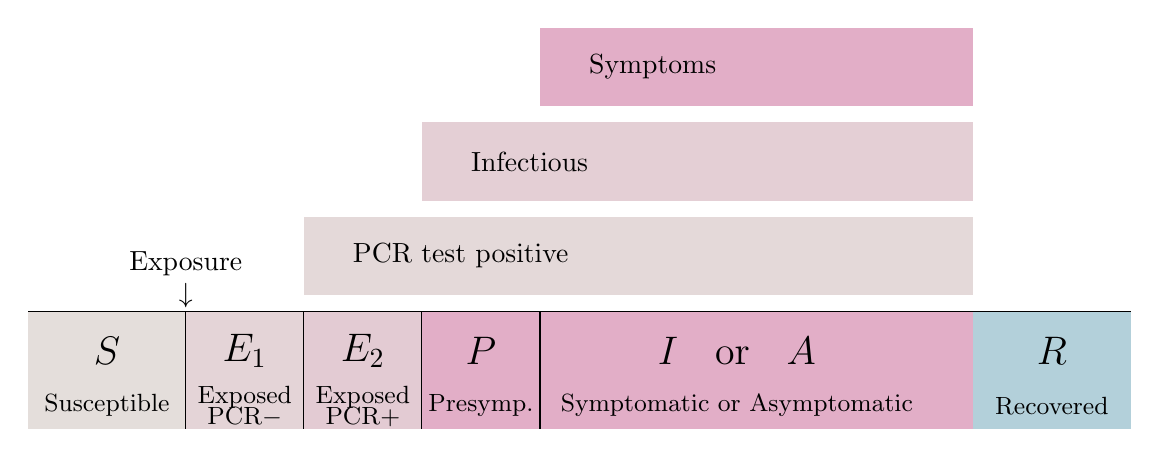
\begin{tikzpicture}
    % \draw[draw = none,fill=susColor!80!infColor] (0,0.2) rectangle (10,1.2);
    % \draw[draw = none,fill=susColor!60!infColor] (1.5,1.4) rectangle (10,2.4); 
    % \draw[draw = none,fill=infColor] (3,2.6) rectangle (10,3.6);
    % \draw[draw = none,fill=infColor] (4.5,3.8) rectangle (10,4.8);

    \draw[draw = none,fill=susColor!90!infColor] (1.5,0.2) rectangle (10,1.2); 
    \draw[draw = none,fill=susColor!70!infColor] (3,1.4) rectangle (10,2.4);
    \draw[draw = none,fill=infColor] (4.5,2.6) rectangle (10,3.6);



    
    % \draw[draw=none,left color=susColor,right color=white] (7,0.2) rectangle (10,1.2);

    
    \draw[fill=susColor,draw=none] (-2,-1.5) rectangle (0,0);
    \draw[fill=susColor!80!infColor,draw=none] (0,-1.5) rectangle (1.5,0);
    \draw[fill=susColor!60!infColor,draw=none] (1.5,-1.5) rectangle (3,0);
    \draw[fill=infColor,draw=none] (3,-1.5) rectangle (4.5,0);
    \draw[fill=infColor,draw=none] (4.5,-1.5) rectangle (10,0);
    % \draw[left color=infColor,right color=infColor,draw=none] (4.5,-1.5) rectangle (10,0);
    \draw[fill=recColor,draw=none] (10,-1.5) rectangle (12,0);
    % \draw[left color=infColor,right color=recColor,draw=none] (10,-1.5) rectangle (12,0);
    % \draw[fill=recColor,draw=none] (10,-1.5) rectangle (12,0);
    % \draw[draw=none,left color=recColor,right color=white](9.5,-1.5) rectangle (13,0);
    % \draw[draw=none,left color=infColor,right color=recColor](10,-1.5) rectangle (13,0);
    

    \draw (-2,0) -- (12,0);
    \draw (0,0) -- (0,-1.5);
    \draw (1.5,0) -- (1.5,-1.5);
    \draw (3,0) -- (3,-1.5);
    \draw (4.5,0) -- (4.5,-1.5);

    \node (S) at (-1,-0.5) {\Large $S$};
    \node (S2) at (-1,-1.2) {\small Susceptible};
    \node (E1) at (0.75,-0.5) {\Large $E_1$};
    \node (E1) at (0.75,-1.1) {\small Exposed};
    \node (E1) at (0.75,-1.35) {\small PCR$-$};
    \node (E2) at (2.25,-0.5) {\Large $E_2$};
    \node (E2) at (2.25,-1.1) {\small Exposed};
    \node (E2) at (2.25,-1.35) {\small PCR+};
    \node (P) at (3.75,-0.5) {\Large $P$};
    \node (P) at (3.75,-1.2) {\small Presymp.};
    \node (IA) at (7,-0.5) {\Large $I$ \; or \; $A$};
    \node (IA) at (7,-1.2) {\small Symptomatic or Asymptomatic};
    \node (R) at (11,-0.5) {\Large $R$};
    \node (R) at (11,-1.2) {\small Recovered};


    \node (exp) at (0,0.2) {$\downarrow$};
    \node (exp2) at (0,0.6) {Exposure};
    \node[anchor=west] (test) at (2,0.7) {PCR test positive};
    \node[anchor=west] (inf) at (3.5,1.9) {Infectious };
    \node[anchor=west] (symp) at (5,3.1) {Symptoms};

    % \draw[rounded corners] (-1,-1) rectangle ()
    % \node[rectangle,rounded corners,fill=susColor,draw,minimum size =  \CompSize cm] (S) at (-1,-1) {\Large $S$};
\end{tikzpicture}

% \begin{tikzpicture}
%     \node[rectangle,rounded corners,fill=susColor,draw,minimum size =  \CompSize cm] (S) at (0,0) {\Large $S$};
%     \node[rectangle,rounded corners,fill=susColor!80!infColor,draw,minimum size =  \CompSize cm] (E1) at (\cd,0) {\Large $E_1$};
%     \node[rectangle,rounded corners,fill=susColor!60!infColor,draw,minimum size =  \CompSize cm] (E2) at (2*\cd,0) {\Large $E_2$};
%     \node[rectangle,rounded corners,fill=infColor,draw,minimum size =  \CompSize cm] (P) at (3*\cd,0)  {\Large $P$};
%     \node[rectangle,rounded corners,fill=infColor,draw,minimum size =  \CompSize cm] (A) at (4*\cd,0) {\Large $A$};
%     \node[rectangle,rounded corners,fill=infColor,draw,minimum size =  \CompSize cm] (Q) at (3.5*\cd,-\cd)  {\Large $Q$};
%     \node[rectangle,rounded corners,fill=infColor,draw,minimum size =  \CompSize cm] (I) at (3.5*\cd,\cd) {\Large $I$};
%     % \node[rectangle,rounded corners,draw,minimum size =  \CompSize cm] (I) at (4*\cd,\cd) {\Large $I$};
%     \node[rectangle,rounded corners,fill=recColor,draw,minimum size =  \CompSize cm] (Rn) at (5*\cd,0) {\Large $R_n$};
%     \node[rectangle,rounded corners,fill=recColor,draw,minimum size =  \CompSize cm] (Rp) at (6*\cd,0) {\Large $R_p$};


%     \draw [-{Latex[scale=2]}]  (S) -- (E1);
%     \draw [-{Latex[scale=2]}]  (E1) -- (E2);
%     \draw [-{Latex[scale=2]}]  (E2) -- (P);
%     \draw [-{Latex[scale=2]}]  (P) -- (A);
%     \draw [-{Latex[scale=2]}]  (P) -- (I);
%     \draw [-{Latex[scale=2]}]  (E2) -- (Q);
%     \draw [-{Latex[scale=2]}]  (P) -- (Q);
%     \draw [-{Latex[scale=2]}]  (A) -- (Q);
%     \draw [-{Latex[scale=2]}]  (A) -- (Rn);
%     \draw [-{Latex[scale=2]}]  (Q) -- ($(Rp)+(0,-\cd)$) -- (Rp);
%     \draw [-{Latex[scale=2]}]  (I) -- ($(Rp)+(0,\cd)$) -- (Rp);

%     \draw [-{Latex[scale=1]}]  ($(S)!0.5!(E1) + (0,0.8)$) -- ($(S)!0.5!(E1)$);
%     \node at ($(S)!0.5!(E1) + (0,1)$) {$\beta (P+A)$};

%     \node at ($(E1)!0.5!(E2)+(0,0.5)$) {$\gamma$};
%     \node at ($(E2)!0.5!(P)+(0,0.5)$) {$\gamma$};
%     \node at ($(P)!0.5!(A)+(0,0.5)$) {$(1-\rho)\gamma$};
%     \node at ($(P)!0.5!(I)+(-0.25,0.5)$) {$\rho \gamma$};
%     \node at ($(E2)!0.5!(Q)+(0.2,0.2)$) {$\tau$};
%     \node at ($(P)!0.5!(Q)+(0.2,0.2)$) {$\tau$};
%     \node at ($(A)!0.5!(Q)+(-0.2,0.2)$) {$\tau$};
%     \node at ($(A)!0.5!(Rn)+(0,0.5)$) {$\nu$};
%     \node at ($(I)+(1,0.5)$) {$\nu$};
%     \node at ($(Q)+(3,0.5)$) {$\nu$};

% \end{tikzpicture}

\end{document}